
% Template for Elsevier CRC journal article
% version 1.2 dated 09 May 2011

% This file (c) 2009-2011 Elsevier Ltd.  Modifications may be freely made,
% provided the edited file is saved under a different name

% This file contains modifications for Procedia Computer Science

% Changes since version 1.1
% - added "procedia" option compliant with ecrc.sty version 1.2a
%   (makes the layout approximately the same as the Word CRC template)
% - added example for generating copyright line in abstract

%-----------------------------------------------------------------------------------

%% This template uses the elsarticle.cls document class and the extension package ecrc.sty
%% For full documentation on usage of elsarticle.cls, consult the documentation "elsdoc.pdf"
%% Further resources available at http://www.elsevier.com/latex

%-----------------------------------------------------------------------------------

%%%%%%%%%%%%%%%%%%%%%%%%%%%%%%%%%%%%%%%%%%%%%%%%%%%%%%%%%%%%%%
%%%%%%%%%%%%%%%%%%%%%%%%%%%%%%%%%%%%%%%%%%%%%%%%%%%%%%%%%%%%%%
%%                                                          %%
%% Important note on usage                                  %%
%% -----------------------                                  %%
%% This file should normally be compiled with PDFLaTeX      %%
%% Using standard LaTeX should work but may produce clashes %%
%%                                                          %%
%%%%%%%%%%%%%%%%%%%%%%%%%%%%%%%%%%%%%%%%%%%%%%%%%%%%%%%%%%%%%%
%%%%%%%%%%%%%%%%%%%%%%%%%%%%%%%%%%%%%%%%%%%%%%%%%%%%%%%%%%%%%%

%% The '3p' and 'times' class options of elsarticle are used for Elsevier CRC
%% The 'procedia' option causes ecrc to approximate to the Word template
\documentclass[3p,times,procedia]{elsarticle}

%% The `ecrc' package must be called to make the CRC functionality available
\usepackage{ecrc}
\usepackage{hyperref}
\usepackage{amsmath}
\usepackage{subfigure}

%% The ecrc package defines commands needed for running heads and logos.
%% For running heads, you can set the journal name, the volume, the starting page and the authors

%% set the volume if you know. Otherwise `00'
\volume{00}

%% set the starting page if not 1
\firstpage{1}

%% Give the name of the journal
\journalname{Procedia Computer Science}

%% Give the author list to appear in the running head
%% Example \runauth{C.V. Radhakrishnan et al.}
\runauth{Ying Liu, Chao Xiang}

%% The choice of journal logo is determined by the \jid and \jnltitlelogo commands.
%% A user-supplied logo with the name <\jid>logo.pdf will be inserted if present.
%% e.g. if \jid{yspmi} the system will look for a file yspmilogo.pdf
%% Otherwise the content of \jnltitlelogo will be set between horizontal lines as a default logo

%% Give the abbreviation of the Journal.
\jid{procs}

%% Give a short journal name for the dummy logo (if needed)
\jnltitlelogo{Procedia Computer Science}

%% Provide the copyright line to appear in the abstract
%% Usage:
%   \CopyrightLine[<text-before-year>]{<year>}{<restt-of-the-copyright-text>}
%   \CopyrightLine[Crown copyright]{2011}{Published by Elsevier Ltd.}
%   \CopyrightLine{2011}{Elsevier Ltd. All rights reserved}
\CopyrightLine{2017}{The Authors. Published by Elsevier B.V.\newline Selection and/or peer-review under responsibility of ITQM2017}


%% Hereafter the template follows `elsarticle'.
%% For more details see the existing template files elsarticle-template-harv.tex and elsarticle-template-num.tex.

%% Elsevier CRC generally uses a numbered reference style
%% For this, the conventions of elsarticle-template-num.tex should be followed (included below)
%% If using BibTeX, use the style file elsarticle-num.bst

%% End of ecrc-specific commands
%%%%%%%%%%%%%%%%%%%%%%%%%%%%%%%%%%%%%%%%%%%%%%%%%%%%%%%%%%%%%%%%%%%%%%%%%%

%% The amssymb package provides various useful mathematical symbols
\usepackage{amssymb}
%% The amsthm package provides extended theorem environments
%% \usepackage{amsthm}

%% The lineno packages adds line numbers. Start line numbering with
%% \begin{linenumbers}, end it with \end{linenumbers}. Or switch it on
%% for the whole article with \linenumbers after \end{frontmatter}.
%% \usepackage{lineno}

%% natbib.sty is loaded by default. However, natbib options can be
%% provided with \biboptions{...} command. Following options are
%% valid:

%%   round  -  round parentheses are used (default)
%%   square -  square brackets are used   [option]
%%   curly  -  curly braces are used      {option}
%%   angle  -  angle brackets are used    <option>
%%   semicolon  -  multiple citations separated by semi-colon
%%   colon  - same as semicolon, an earlier confusion
%%   comma  -  separated by comma
%%   numbers-  selects numerical citations
%%   super  -  numerical citations as superscripts
%%   sort   -  sorts multiple citations according to order in ref. list
%%   sort&compress   -  like sort, but also compresses numerical citations
%%   compress - compresses without sorting
%%
%% \biboptions{comma,round}

% \biboptions{}

% if you have landscape tables
\usepackage[figuresright]{rotating}

% put your own definitions here:
%   \newcommand{\cZ}{\cal{Z}}
%   \newtheorem{def}{Definition}[section]
%   ...

% add words to TeX's hyphenation exception list
%\hyphenation{author another created financial paper re-commend-ed Post-Script}

% declarations for front matter

\begin{document}

\begin{frontmatter}

%% Title, authors and addresses

%% use the tnoteref command within \title for footnotes;
%% use the tnotetext command for the associated footnote;
%% use the fnref command within \author or \address for footnotes;
%% use the fntext command for the associated footnote;
%% use the corref command within \author for corresponding author footnotes;
%% use the cortext command for the associated footnote;
%% use the ead command for the email address,
%% and the form \ead[url] for the home page:
%%
%% \title{Title\tnoteref{label1}}
%% \tnotetext[label1]{}
%% \author{Name\corref{cor1}\fnref{label2}}
%% \ead{email address}
%% \ead[url]{home page}
%% \fntext[label2]{}
%% \cortext[cor1]{}
%% \address{Address\fnref{label3}}
%% \fntext[label3]{}

\dochead{Information Technology and Quantitative Management (ITQM 2017)}
%% Use \dochead if there is an article header, e.g. \dochead{Short communication}
%% \dochead can also be used to include a conference title, if directed by the editors
%% e.g. \dochead{17th International Conference on Dynamical Processes in Excited States of Solids}

\title{Hybrid Learning Network:\\ 
	A Novel Architecture for
	Fast Learning}

%% use optional labels to link authors explicitly to addresses:
%% \author[label1,label2]{<author name>}
%% \address[label1]{<address>}
%% \address[label2]{<address>}

\author[u1,u2]{Ying Liu}
\author[u1]{Chao Xiang}

\address[u1]{School of Computer 
	and Engineering, University of 
	Chinese Academy of Sciences, 
	Beijing, 100190 China}
\address[u2]{Key Lab of Big Data
	Mining and Knowledge Management,
	Chinese Academy of Sciences,
	Beijing, 100190 China}

\begin{abstract}
%% Text of abstract
There're many effective architectures 
of the artificial neural network(ANN).
For which the training is a hard work.
The cost for training an ANN increases
exponentially when the ANN gets deeper 
or wider. 
We therefore propose a novel 
architecture, the Hybrid Learning
Network(HLN), to achieve a fast learning 
with good stablity.
The HLN can learn from both
labeled data and unlabeled data
at the same time in a hybrid
learning manner.
It uses a Self Organizing Map unified
by the specially designed nonlinear
function as the sparsity mask 
for a hidden layer to improve 
the training speed.
We experiment our architecture on 
a synthetic dataset to test its 
regression capability against the
traditional architecture, the result 
is promising.
We also experiment on the well-known
MNIST dataset, it demonstrates an 
even more impressive learning eciency 
by up to $40\times$ speed-up on training.
It indicates that our architecture performs
better on handling larger datasets and 
tackling larger problems.
\end{abstract}

\begin{keyword}
HLN; hybrid learning; neural network; sparsity mask; SOM; MNIST; fast learning

%% keywords here, in the form: keyword \sep keyword

%% PACS codes here, in the form: \PACS code \sep code

%% MSC codes here, in the form: \MSC code \sep code
%% or \MSC[2008] code \sep code (2000 is the default)

\end{keyword}

\end{frontmatter}

\correspondingauthor[*]{Corresponding author. Tel.: +86-183-0114-2368;}
\email{xiangchao215@mails.ucas.ac.cn}

%%
%% Start line numbering here if you want
%%
% \linenumbers

%% main text
\section{Introduction}
\label{main}
Since the first mathematical model 
of the artificial neural network(ANN) was 
proposed in 
1943\cite{mcculloch1943logical}, 
lots of different architectures 
have been proposed
to develop the model, such as 
the Convolutional Neural Network(CNN) 
for image recognition
\cite{krizhevsky2012imagenet}, 
the Recurrent Convolutional Neural 
Network(R-CNN) for object 
detection in videos
\cite{girshick2015fast}, 
and the Long Short Term Memory(LSTM)
for speech recognition
\cite{graves2013hybrid}, etc. 
These specially designed neural 
networks are trained by 
a few ecient methods such as
the stochastic gradient 
descent(SGD)\cite{bottou2010large}. 
Such architectures
suit well for their specific 
applications but may have plain 
or worse performances on others, 
and their best performances 
rely heavily on the hyperparameter 
configuration. Therefore
a relatively universal 
architecture that enables equal 
or similar performances among 
varied applications is in real demand.

Although a number of
different neural network architectures
have been proposed in the past years,
literally all of them can be classifed
into 3 categories, supervised
\cite{lecun1990handwritten}, 
unsupervised
\cite{vincent2010stacked}, 
and semi-supervised learning
\cite{chapelle2009semi}.
In supervised learning, 
one can only train a model on
labeled samples. However in real 
applications, labeling a large 
dataset is infeasible as a result
unlabeled samples are 
the major. To make use of 
unlabeled data, a few 
unsupervised training algorithms 
emerged. These unsupervised learning
methods attempt to produce an optimized 
parameter initialization
\cite{le2013building}.
Thus, such unsupervised techniques 
can only be applied before the 
supervised training phase. Once 
the supervised begins, 
unsupversied learning will quit.
Semi-supervised learning
allows the model to learn from
both labeled and unlabeled samples
at the same time, where a
regularizer is embedded in
the supervised optimizing object,
and generally a balance constraint is
required to avoid the trival solution
\cite{socher2011semi}.
Such an enhanced learner brings more 
hyperparameters(such as the balance 
constraint), making it even more 
difficult to search for the best 
settings for current architectures. 
Additionally, this integration manner 
makes it impossible to separate the 
two learners as the semi-supervised 
regularizer is built on the supervised 
learner, and therefore an 
early supervised training alone with 
profound labeled data is necessary
before the semi-supervised learning 
starts.

Therefore in the paper, we introduce 
a new architecture that combines the
supervised and unsupervised learning
requiring no extra techniques in
training. Our architecture, the Hybrid
Learning Network(HLN), consists of 
stacked hybrid learning layers, 
each of which
embeds a Self Organizing
Map(SOM). In the similar manner of 
backpropagation, HLNs
demonstrate higher learning
capability and stablity. 

%\subsection{Our contributes}
The main contributions of our work are:
\begin{itemize}
\item
	HLN is proposed as a hybrid learning
	architecture to learn both unlabeled 
		and labeled data simultaneously.
		HLN overcomes
the problem of traditional 
semi-supervised learning methods which 
requires
an early standalone training for the
supervised learner.
\item A SOM-embedding layer structure is 
	designed to learn a cluster 
mapping function from unlabeled data
		to speed up the supervised
		learning from labeled
data.
\item A nonlinear function $h(x)$,
	is proposed to 
		measure the state of a
		SOM in each iteration of the 
		training, and then determine 
		a sparsity
		mask for every hidden layer.
\end{itemize}
Our proposed HLN is implemented in 
Python and all
our code and results of experiments
are available at
\url{https://github.com/hiroki-kyoto/hybrid-learning-net}.

%\subsection{The organization of this artical}
The rest of the paper is organized
as follows.
In section 2 we introduce existing
semi-supervised algorithms for neural
network models and SOM.
In section 3, we present our novel
architecture HLN and how to
embed SOMs into deep architectures of
neural networks.
In section 4 we explain the 
training theory for HLNs.
Section 5 presents the experimental
results, and the
last section concludes our work.

\section{Related work and background
Knowledge}
\label{sec:related_work}
\subsection{Semi-supervised learning for
neural network}
A key assumption in semi-supervised 
algorithms, is the 
structure assumption: two samples with 
similar distribution on the same mapping 
structure tend to have high probability 
belonging to the same class. Based on 
this assumption, one can use large 
unlabeled data to uncover such 
structures. There're already a few 
algorithms dedicated to it,
such as cluster kernels
\cite{chapelle2003cluster},
Low Density Separation(LDS)
\cite{chapelle2005semi},
label propagation
\cite{zhu2002learning},
etc.
In such algorithms, designing 
a regularizer
to enable the model to learn 
the representation
or structure of raw data
becomes the key point.

Let's firstly focus on the 
general algorithm
description of semi-supervised learning.
Given a set of unlabeled samples,
$\mathbf{X}=\{\mathbf{x}_1,\cdots,
\mathbf{x}_N\}(\mathbf{x}\in\mathbb{R}^d)$,
and the similarity labels between any
$\mathbf{x}_i$ and $\mathbf{x}_j$,
$\mathbf{W}=\{W_{ij}|i,j=1,\cdots,N\}$,
our goal is to find the best 
embedding function,$f(\mathbf{x})$, 
for each sample $\mathbf{x}_i$, 
in order to minimize:
\begin{equation}
\Delta_{f}=
	\sum^{N}_{i=1}
	\sum^{N}_{j=1}
	L\left(
	f(\mathbf{x}_i),
	f(\mathbf{x}_j),
	W_{ij}
	\right)
\label{eq:1}
\end{equation}
where,
\begin{itemize}[]
\item $L(\cdot)$ is the loss 
function of 3 
variables: 
$\left<
		f(\mathbf{x}_i),
		f(\mathbf{x}_j),
		W_{ij}
		\right>$.
For example, if Euclidean distance
is used,
		$$L\left(
		f(\mathbf{x}_i),
		f(\mathbf{x}_j),
		W_{ij}
		\right) = 
		\left(
		\|f(\mathbf{x}_i)-
		f(\mathbf{x}_j)
		\|-W_{ij}
		\right)^2$$
\item $f(\mathbf{x})\in\mathbb{R}^n$ 
is the 
embedding function, 
trying to produce an output
vector for $\mathbf{x}_i$, 
similar to that 
for $\mathbf{x}_j$ with $W_{ij}=0$,
and disimilar with $W_{ij}=1$.
\item $W_{ij}\in \mathbb{R}$ is 
the similarity 
label of the sample pair
$\left<
		\mathbf{x}_i,
		\mathbf{x}_j
		\right>$ from $\mathbf{X}$.
\end{itemize}
As a result, the overall optimization 
object is
\begin{equation}
	\arg \min 
	\sum_i
	\ell\left(
	f(\mathbf{x}_i),
	\mathbf{\hat{y}}_i
	\right)+
	\lambda\Delta_f
\end{equation}
where $\ell(\cdot)$ is the loss
function for supervised learning.
$\lambda$ is proposed 
as the balance 
coefficient to embed
the semi-supervised 
regularizer $\Delta_f$.

\subsection{Self Organizing Map}
Self Organizing Map is an effective 
method for the visualization of 
high-dimensional data. 
It can also be used 
as an automatic clustering method. 
The SOM consists of a two-dimensional 
regular grid of nodes. 
The models are automatically 
organized into a meaningful 
two-dimensional order in which 
similar models are closer to
each other in the grid than 
the more dissimilar
ones\cite{kohonen1998self}.
Rules used to update models are:
\begin{equation}
	\mathbf{m}_i(t+1)=\mathbf{m}_i(t)+
	h_{c(x),i}\left(
	\mathbf{x}(t)-\mathbf{m}_i(t)
	\right)
	\label{eq:8}
\end{equation}
and the learning rate is 
dynamically determined as
\begin{equation}
	h_{c(x),i} = \alpha(t)\exp\left(
	-\frac{\|\mathbf{r}_i-\mathbf{r}_c\|^2}
	{2\sigma^2(t)}
	\right)
	\label{eq:9}
\end{equation}
where $\mathbf{m}_i\in\mathbb{R}^n$ 
denotes the $i^{th}$ model vector, 
$\mathbf{x}$ is an input pattern,
$c(x)$ relates to the best match 
vector index
in $\mathbf{m}$ for input 
pattern $\mathbf{x}$,
and $\alpha(t)$ is a learning rate 
that decreases as the
training preceeds.
$\mathbf{r}$ denotes the model vector 
location in 
the map, and $\sigma(t)$ 
corresponds to the 
width of the neighborhood 
function, which 
also decreases monotonically 
with the regression steps.

\section{Hybrid Learning Network}
Hybrid Learning Network is a novel
architecture aiming at 
enhancing arbitrary networks
on their training eciency and
stablity.
Each hidden layer in HLN architecture 
is embedded with a SOM. For the 
simplest case where neurons are fully connected, 
the traditional
architecture, called Fully 
Connected Network(FCN) architecture,
is presented in Figure~\ref{fig:1:a}.
The proposed HLN architecture is
presented in Figure~\ref{fig:1:b}.

\begin{figure}
	\centering
	\subfigure[The FCN architecture]{
		\label{fig:1:a}
		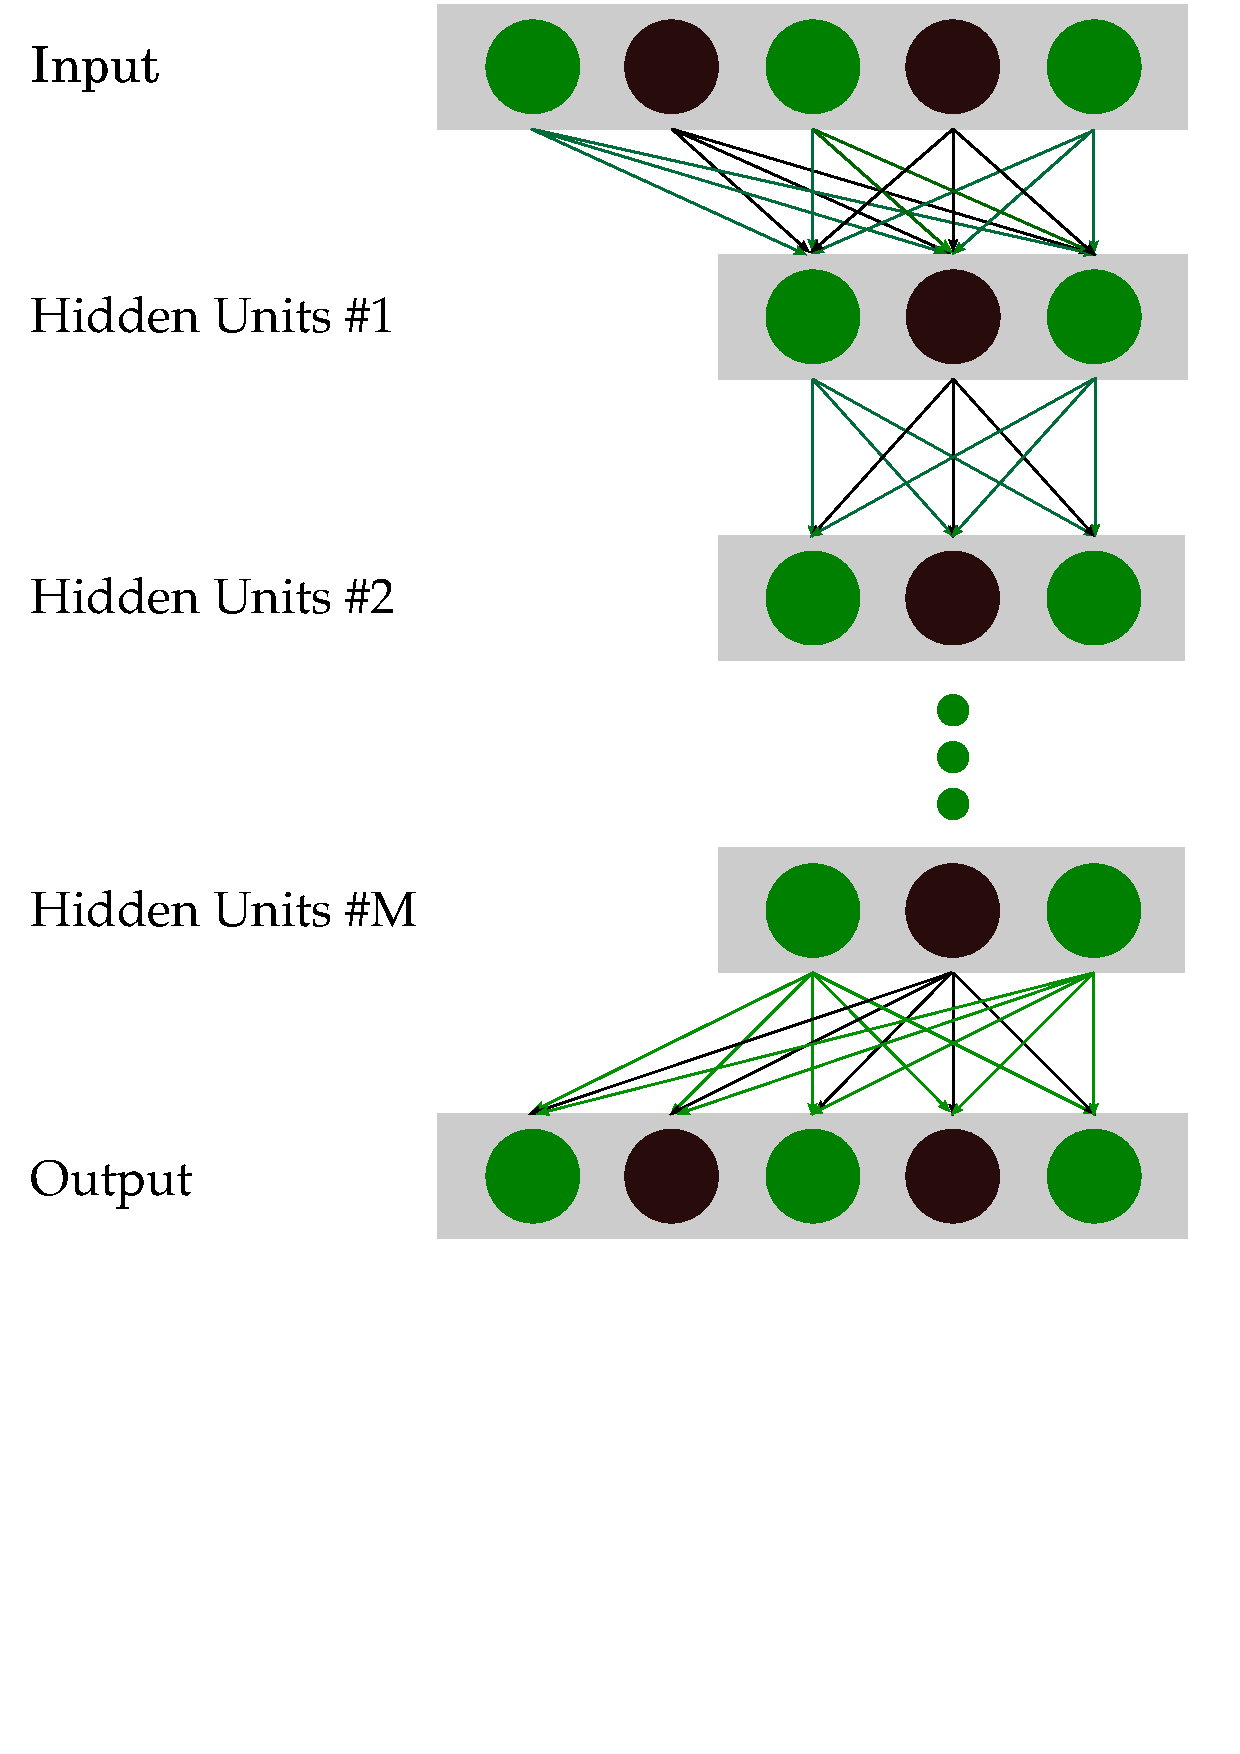
\includegraphics[width=2in]{FCN}}
	\hspace{0.2in}
	\subfigure[The HLN architecture]{
		\label{fig:1:b}
		\includegraphics[width=2in]{HLN}}
	\caption{The left is FCN architecture, 
	the right is HLN architecture.
	The big solid circles are the 
	neurons, the medium ones are the 
	middle states of neurons, and 
	the small ones are the vector maps 
	$\mathbf{m}^k$ of SOMs, finally the 
	tiny ones are the function modules.
	The parts omitted refers to repeating
	hidden layers connected in same way.}
	\label{fig:1}
\end{figure}

In HLN architecture,
we propose $h(x)$, 
an unifying function for 
SOM, to convert pattern disimilarity
$\|\mathbf{x}-\mathbf{m}_i\|$ to
a semi-supervised learning factor for
different hidden units. 
The semi-supervised
learning factors act as a 
dynamic neuron activation 
sparsity mask for 
each hybrid learning layer.
It works in the similar manner  
as the Dropout 
technique\cite{srivastava2014dropout}, 
enabling the neural networks 
to improve the model robustness 
and prevent
overfitting by learning 
their submodels for 
each batch. However, HLN differs from 
techniques like Dropout because 
HLN does not generate sparsity with 
randomness. HLN uses the SOM
to unsupervisedly learn 
the \emph{static}
policy of the neuron-activation 
distribution for
each hidden layer, the network 
sparsity generator thereby
will stablize with training 
steps, and the
randomness in sparsity will 
disappear automatically.
We propose $h(x)$ as follows,
\begin{equation}
	\delta_{max} = \max_i\left(
	\|\mathbf{m}_i-\mathbf{x}\|+\epsilon
	\right)
	\label{eq:10}
\end{equation}
\begin{equation}
	\delta_{min} = \min_i\left(
	\|\mathbf{m}_i-\mathbf{x}\|+\epsilon
	\right)
	\label{eq:11}
\end{equation}
where $\delta_{max}$ is the maximum 
disimilarity
between an arbitrary vector 
$\mathbf{m}_i$
and the input pattern vector $\mathbf{x}$,
$\delta_{min}$ is the minimum one.
The scale of all disimilarities is
\begin{equation}
	\delta_{scale} = 
	\frac{\mathbf{\delta}_{min}}
	{\mathbf{\delta}_{max}-
	\mathbf{\delta}_{min} + \epsilon}
	\label{eq:12}
\end{equation}
We then unify the disimilarities 
and convert them into sparsity 
mask as
\begin{equation}
	h(x)|_{x=\|\mathbf{m}_i-\mathbf{x}\|}=
	\frac{\delta_{max}\cdot\delta_{scale}}
	{\left\|\mathbf{m}_i-\mathbf{x}\right\|
	+\epsilon}-\delta_{scale}
	\label{eq:13}
\end{equation}
where $\mathbf{m}_i$ and $\mathbf{x}$ 
is the same way defined as in 
equation~(\ref{eq:8}).
$\epsilon$ is set at a small constant
value, such as $\epsilon=10^{-5}$,
to avoid 
\emph{division-by-zero} errors,
which rarely happens. 
Notice that
if any other metric is preferred, 
we can
always replace the pattern 
disimilarity
$\|\mathbf{m}_i-\mathbf{x}\|$ with 
other forms.
$f(s,o)$ is the function to combine the 
sparsity mask $s$ generated by $h(\cdot)$ 
and the fully connected linear summation 
output $o$. In most cases, we use the
simple multiplication as the operator,
\begin{equation}
	f(s,o) = s\cdot o = 
	h\left(
	\left\|
	\mathbf{m}_i-\mathbf{y^{k-1}}
	\right\|
	\right)
	\cdot
	\sum_j
	\left(
	w_j^{k,i}y_j^{k-1}
	\right)
	+b^{k,i},k>1
	\label{eq:14}
\end{equation}
As shown in Figure~\ref{fig:1:b}, 
$f(\cdot) $ is followed 
by an activation function, which could 
be any 
arbitrary nonlinear function that 
takes 
only one dimension input and 
outputs a 
single real value, 
such as the sigmoid function, 
$tanh(x)$ and ReLU. 
With the new 
architecture, 
we update the forward computing
rules as 
\begin{equation}
	y_i^k(\mathbf{x})=
	\sigma\left(
	h\left(
	\left\|
	\mathbf{m}_i^k-y^{k-1}(\mathbf{x})
	\right\|
	\right)\cdot
	\sum_j\left(
	w_j^{k,i}y_j^{k-1}(\mathbf{x})
	\right) + b^{k,i}
	\right), k>1
	\label{eq:15}
\end{equation}
and for the first hybrid learning layer,  
\begin{equation}
	y_i^1(\mathbf{x})=
	\sigma\left(
	h\left(
	\left\|
	\mathbf{m}_i^1-\mathbf{x}
	\right\|
	\right)\cdot
	\left(
	\sum_j w_j^{1,i}x_j
	\right) + b^{1,i}
	\right)
	\label{eq:16}
\end{equation}
where $m^k_i$ denotes the $i^{th}$ 
vector in the $k^{th}$ SOM of 
the net(all indexes start from 1), 
and $\sigma$ is a nonlinear 
activation function.

\section{HLN Training}
Let's compare the theories between
HLN and the general model mentioned 
in section~\ref{sec:related_work}.
Existing semi-supervised algorithms
include a regularizer into the supervised
learning optimizing object, making it 
impossible to train both of
the supervised learner and the 
unsupervised one
separatedly. As analyzed before, 
performance
of such regularizer solutions depends 
on the
standalone supervised pretraining 
which requires profound labeled data.
However, in our proposed architecture 
HLN, we assign
each of the learning methods a 
completely
separated optimizing object, with no 
priority
orders restricted.

For the supervised learning, we may 
have such an optimizing object,
\begin{equation}
	\arg \min_g \sum_{i=1}^L\ell\left(
	g(\mathbf{x}_i),
	\mathbf{\hat{y}}_i
	\right)
	\label{eq:17}
\end{equation}
where $g(\mathbf{x})$ is the
function describing
the mapping from the input 
$\mathbf{x}\in\mathbb{R}^d$ to the 
output
$\mathbf{y}\in\mathbb{R}^n$, 
parameterized with
the neural connection 
weights $\mathbf{W}$ and 
the biases $\mathbf{b}$ for all 
non-input 
layer neurons in the HLN 
architecture.
Equation~\ref{eq:17} becomes the 
Equation~\ref{eq:18} when Enclidean 
metric is applied as the loss function.
\begin{equation}
	\arg \min_{\mathbf{W},\mathbf{b}}
	\frac{1}{2}
	\sum_{i=1}^L
	\left\|
	y^k(
	\mathbf{x}_i)\big|_{\mathbf{W},\mathbf{b}}-
	\mathbf{\hat{y}}_i
	\right\|^2
	\label{eq:18}
\end{equation}
For the unsupervised learning, 
the optimizing
objects are
\begin{equation}
	\arg \min_{\mathbf{m}^k}
	\sum_i^{L+U}
	\left(
	\min_j\left(
	\left\|
	\mathbf{m}^k_j-\mathbf{x}^k_i
	\right\|
	\right)
	\right),\quad k=1,2,\cdots
	\label{eq:19}
\end{equation}
with the predefined notation:
\begin{equation}
	\mathbf{x}_i^k=
	\left\{
		\begin{aligned}
			\mathbf{x}_i,\quad & k=1\\
			y^{k-1}(\mathbf{x}_i),\quad & k>1
		\end{aligned}
	\right.
	,\quad \mathbf{x}_i\in L+U
	\label{eq:20}
\end{equation}

For a net with $M$ hybrid learning layers,
there should be 1 supervised optimizing
object
and $M$ unsupervised optimizing objects.
Although a multi-objective problem 
may not 
have a global solution, in HLNs, since
each object is optimized in its 
own isolated
parameter space, 
each optimizing object
has its own global 
optimization 
solution.

Using the well-known Back 
Propagation(BP)
algorithm, we can obtain parameter 
updating
rules for HLN training.
We focus on the difference between HLN
and the original BP algorithm for 
the FCN model.
Let's denote the linear summation 
for $i^{th}$ unit
in $k^{th}$ layer as $o_i^k$, then
the linear summations of hybrid learning
layers are (with $\mathbf{y}^0=\mathbf{x}$):
\begin{equation}
	o_i^k =
	h\left(
	\left\|
	\mathbf{m}_i^k-\mathbf{y}^{k-1}
	\right\|
	\right)
	\sum_j 
	W_j^{k,i}
	y_j^{k-1},
	\quad k=1,2,\cdots,M
	\label{eq:23}
\end{equation}
Apply the non-linear activation 
function, for example, the sigmoid
function:
\begin{equation}
	\frac{\partial E}
	{\partial o_i^k}=
	\frac{\partial E}
	{\partial y_i^k}
	\sigma'(o_i^k)=
	\frac{\partial E}
	{\partial y_i^k}
	y_i^k\left(
	1-y_i^k
	\right),
	\quad k=1,2,\cdots,M+1
	\label{eq:24}
\end{equation}
Thus the recursive layer gradient 
computing is shown in 
Equation~\ref{eq:25}.
\begin{equation}
	\frac{\partial E}
	{\partial y_i^{k-1}}=\sum_j
	\frac{\partial E}
	{\partial o_j^k}
	h\left(
	\left\|
	\mathbf{m}_j^k-
	\mathbf{y}^{k-1}
	\right\|
	\right)
	W_j^{k,i}
	\quad k=1,2,\cdots,M
	\label{eq:25}
\end{equation}
The partial error gradients for the
connection parameters $\mathbf{W}$
are shown in Equation~\ref{eq:27}.
\begin{equation}
	\frac{\partial E}
	{\partial W_j^{k,i}}=\sum_i
	\frac{\partial E}
	{\partial o_i^k}
	h\left(
	\left\|
	\mathbf{m}_i^k-
	\mathbf{y}^{k-1}
	\right\|
	\right)
	y_i^{k-1},
	\quad k=1,2,\cdots,M
	\label{eq:27}
\end{equation}
The partial error gradients 
on biases are presented in 
Equation~\ref{eq:29}.
\begin{equation}
	\frac{\partial E}
	{\partial b^{k,i}}=
	\frac{\partial E}
	{\partial o_i^k}
	\frac{\partial o_i^k}
	{\partial b^{k,i}}=
	\frac{\partial E}
	{\partial o_i^k}
	\times 1,
	\quad k=1,2,\cdots,M+1
	\label{eq:29}
\end{equation}
Therefore we can iterate 
recursively along layers using
Equation~(\ref{eq:23})(\ref{eq:24})
(\ref{eq:25})(\ref{eq:27})
(\ref{eq:29}) to 
update all the parameters of 
the supervised 
training, and the corresponding 
parameter updating rules 
for the unsupervised 
training are shown in 
Equations~(\ref{eq:8})(\ref{eq:9}).

\section{Empirical Study}
\subsection{Synthetic data}
A synthetic dataset is generated. 
It maps a set of
2-dimension vectors into 3 classes, 
where
$3.5\%$ of the noise is included
to simulate a real application.
We then apply the data to an instance
of HLN and FCN.
In both networks, we only use a single
hidden layer.
Figure~\ref{fig:2}-\ref{fig:3} 
present the progress of the accuracy 
as the number of epoches increases.

\begin{figure}[h]
	\centering
	\subfigure[]{
		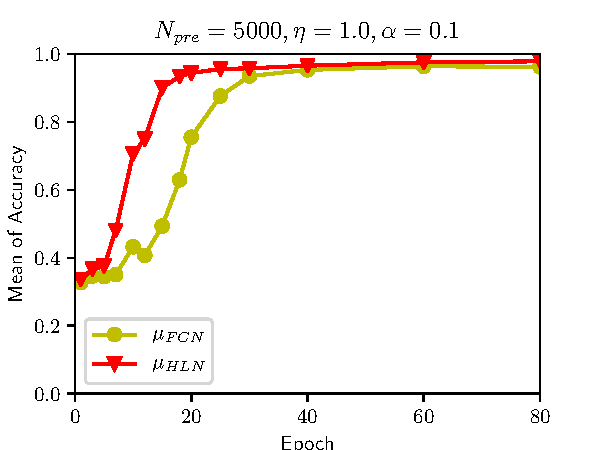
\includegraphics[width=55mm]{mean_accuracy0}
		\label{fig:2:a}
	}
	\hspace{-8mm}
	\subfigure[]{
		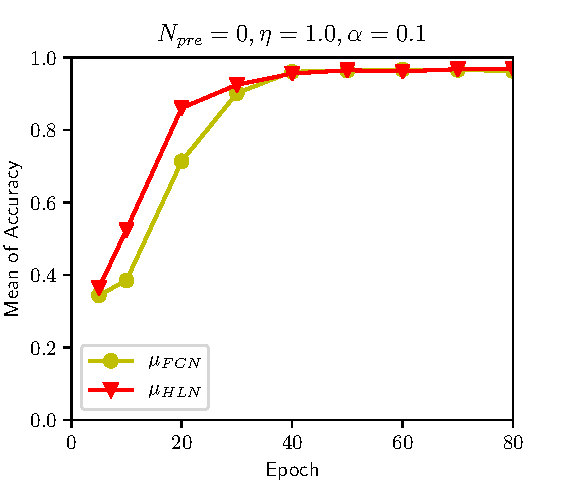
\includegraphics[width=55mm]{mean_accuracy1}
		\label{fig:2:b}
	}
	\hspace{-8mm}
	\subfigure[]{
		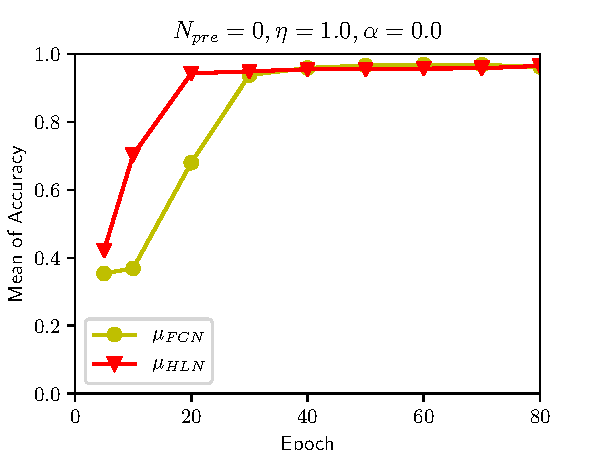
\includegraphics[width=55mm]{mean_accuracy2}
		\label{fig:2:c}
	}
	\caption{
		Mean of 
		accuracy on the synthetic data:
		$\mu$ is the mean accuracy for
		multiple replays with the same
		configuration.
		$N_{pre}$ is the number of
		unlabeled samples
		for pretraining, $\eta$
		is the initial learning rate,
		$\alpha$ is the decay factor of
		learning rate $\eta(t)$.
		}
	\label{fig:2}
\end{figure}

\begin{figure}[h]
	\centering
	\subfigure[]{
		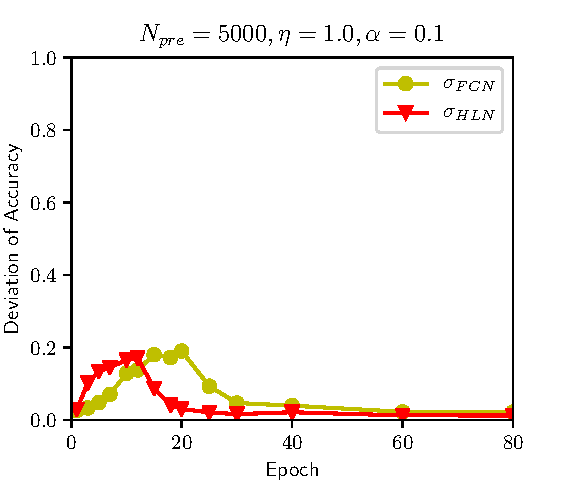
\includegraphics[width=55mm]{devi_accuracy0}
		\label{fig:3:a}
	}
	\hspace{-8mm}
	\subfigure[]{
		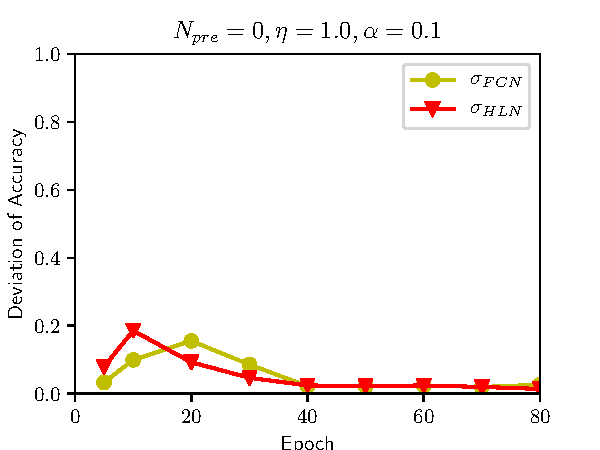
\includegraphics[width=55mm]{devi_accuracy1}
		\label{fig:3:b}
	}
	\hspace{-8mm}
	\subfigure[]{
		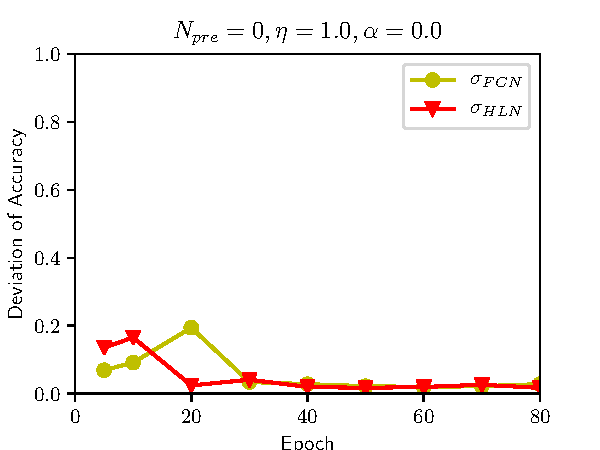
\includegraphics[width=55mm]{devi_accuracy2}
		\label{fig:3:c}
	}
	\caption{
		Deviation of
		accuracy on the synthetic data:
		the deviation takes the form as
		$\delta$ is the deviation of
		multiple replays with the same
		configuration 
		$\delta=\sum_1^N(\gamma_i-\mu)/N$
		, where $\gamma_i$ is the
		accuracy of $i^{th}$ replay.
		}
	\label{fig:3}
\end{figure}

In the experiment,
we split the data into two partitions, 
one for the training of two
architectures and the another for
testing with the train/test ratio 0.8.
Considering the possible impact from
the parameter initialization,
we replay the complete workflow
of training and testing with varied
random parameter initializations
for every net with different 
configurations.
In Figure~\ref{fig:2}, It is evident
that networks with our HLN 
architecture win over networks without 
HLN in all cases.
The experimental results indicate:
\begin{itemize}
	\item HLN architecture 
		learns much faster than
		FCN.
	\item The pretraining
		with unlabeled data does improve 
		the performance of HLN, though 
		the improvement in accuracy
		is not evident.
	\item A constant learning rate is
		more advisable than a varying
		learning rate.
\end{itemize}

Figure~\ref{fig:3} shows that HLN
stablized quickly in all cases,
while FCN requires more training
to stablize. It indicates that 
HLN is more robust to parameter
initialization.
\subsection{MNIST}
Our experiments on the well-known MNIST
benchmark demonstrated even
greater enhencement
over the traditional architecture.
Moreover the advantage of HLN is 
more evident
with higher input dimension
and deeper network. 
To enable the input dimension variation,
a max-pooling is applied before the input
of a neural net. The MNIST dataset
provides 50,000 images for training and 
10,000 images for testing, with each image
resized as $28\times 28$ of pixels. 
A max-pooling with the kernel of 
$2\times 2$
leads to a input dimension of 196, and
particularly a max-pooling with the
kernel $1\times 1$ will keep the original
input dimension as 784. All networks used
are configured as in 
Figure~\ref{fig:1}.

\begin{figure}[h]
	\centering
	\subfigure[]{
		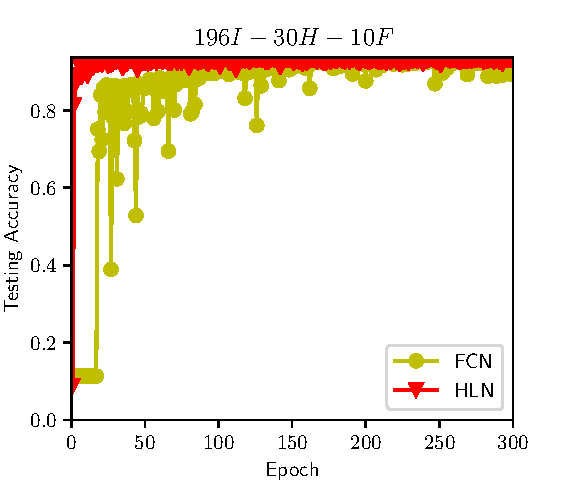
\includegraphics[width=60mm]{mnist_testing_accuracy_1}
		\label{fig:4:a}
	}
	\hspace{-5mm}
	\subfigure[]{
		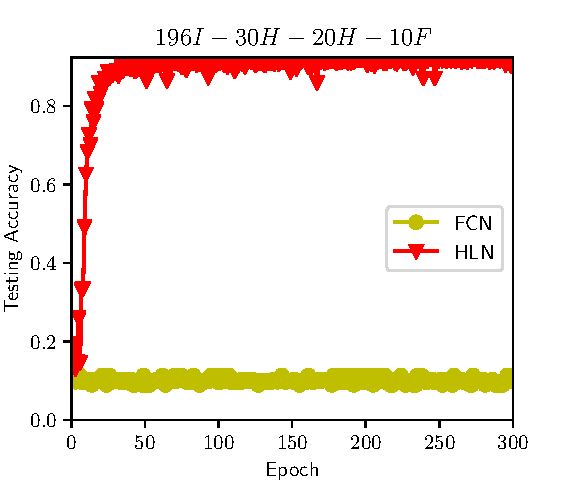
\includegraphics[width=60mm]{mnist_testing_accuracy_2}
		\label{fig:4:b}
	}
	\subfigure[]{
		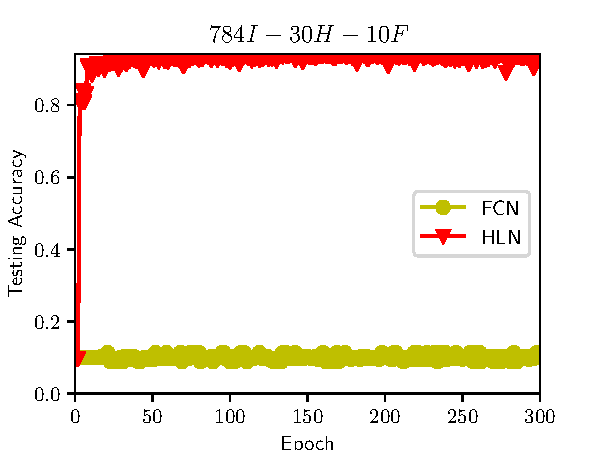
\includegraphics[width=60mm]{mnist_testing_accuracy_3}
		\label{fig:4:c}
	}
	\hspace{-5mm}
	\subfigure[]{
		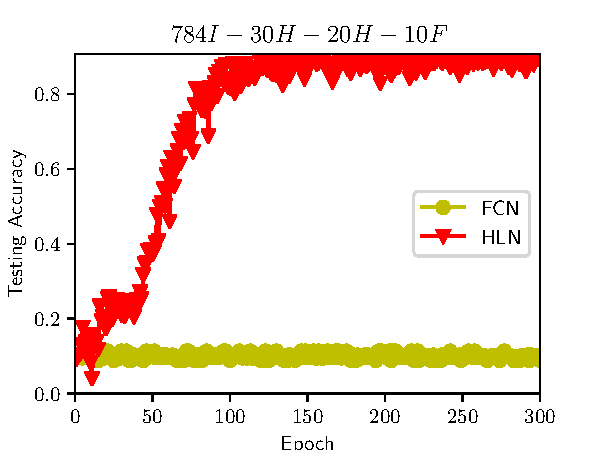
\includegraphics[width=60mm]{mnist_testing_accuracy_4}
		\label{fig:4:d}
	}

	\caption{
		Accuracy on 
		MNIST with 4 different network
		models: 
		$196I$ denotes
		the input layer of dimension 196, 
		$30H$ denotes the hidden layer
		of dimension of 30, and $10F$ 
		denotes
		the fully connected output layer 
		of dimension 10.
		}
	\label{fig:4}
\end{figure}

\begin{figure}[h]
	\centering
	\subfigure[]{
		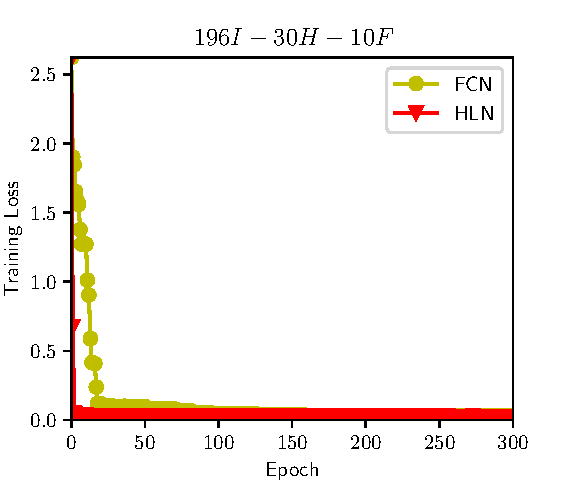
\includegraphics[width=60mm]{mnist_training_loss_1}
		\label{fig:5:a}
	}
	\hspace{-5mm}
	\subfigure[]{
		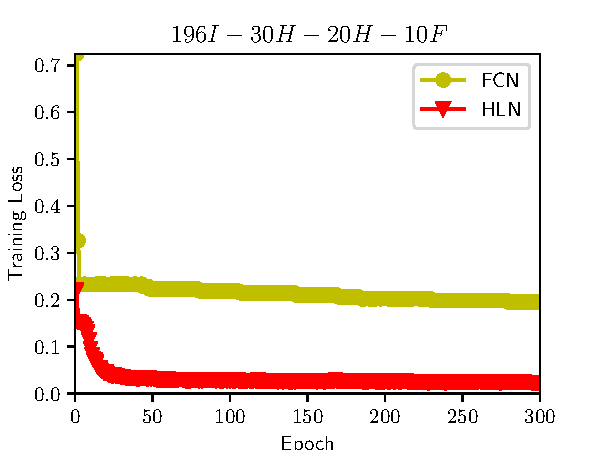
\includegraphics[width=60mm]{mnist_training_loss_2}
		\label{fig:5:b}
	}
	\subfigure[]{
		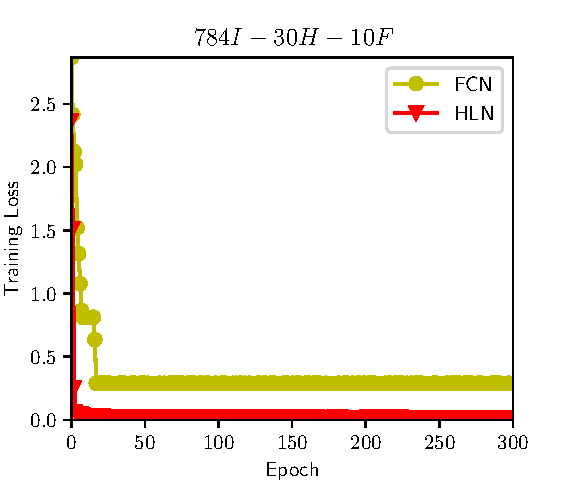
\includegraphics[width=60mm]{mnist_training_loss_3}
		\label{fig:5:c}
	}
	\hspace{-5mm}
	\subfigure[]{
		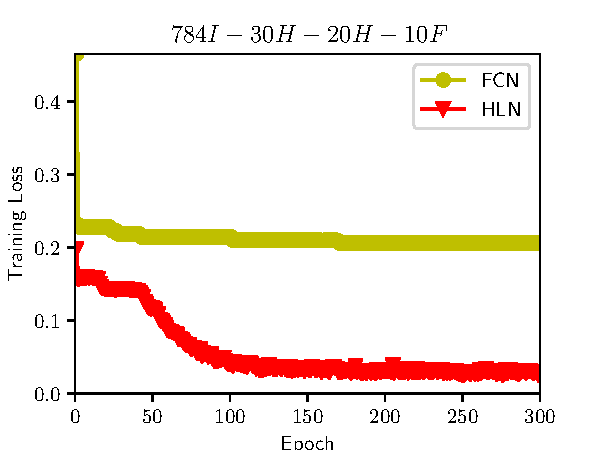
\includegraphics[width=60mm]{mnist_training_loss_4}
		\label{fig:5:d}
	}

	\caption{
		Training loss on 
		MNIST with 4 different network 
		models
		}
	\label{fig:5}
\end{figure}

\begin{figure}[h]
	\centering
	\subfigure[]{
		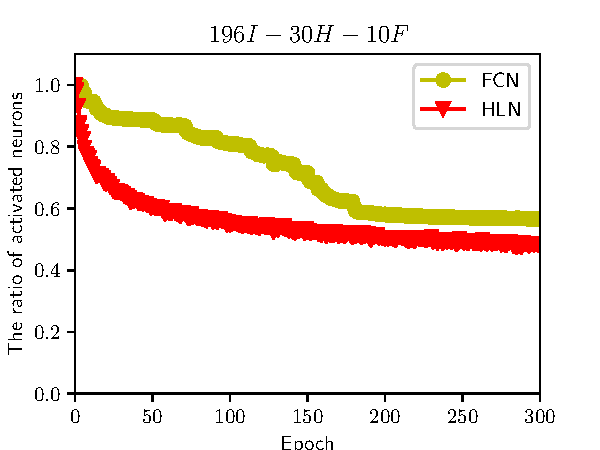
\includegraphics[width=60mm]{mnist_training_sparsity_1}
		\label{fig:6:a}
	}
	\hspace{-5mm}
	\subfigure[]{
		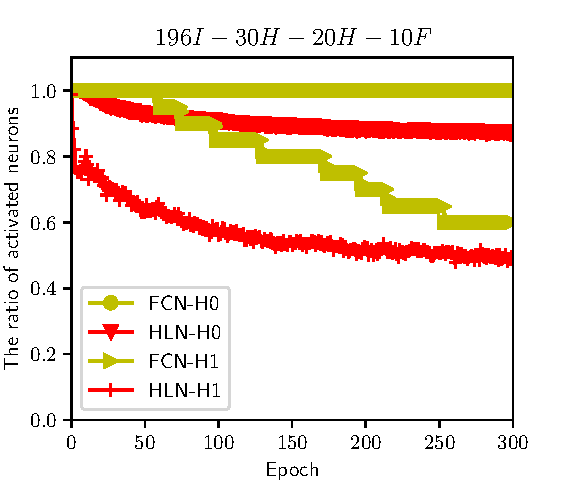
\includegraphics[width=60mm]{mnist_training_sparsity_2}
		\label{fig:6:b}
	}
	\subfigure[]{
		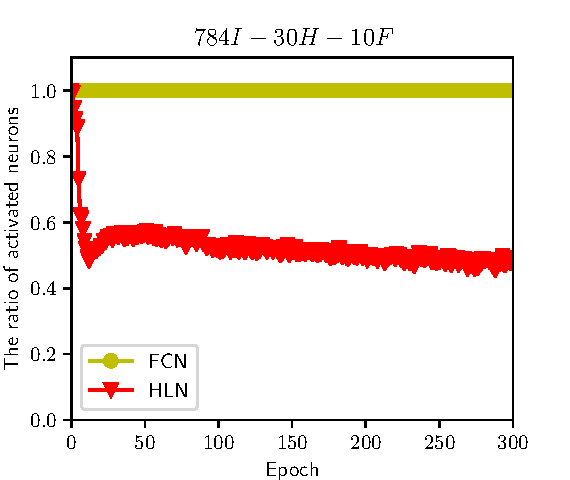
\includegraphics[width=60mm]{mnist_training_sparsity_3}
		\label{fig:6:c}
	}
	\hspace{-5mm}
	\subfigure[]{
		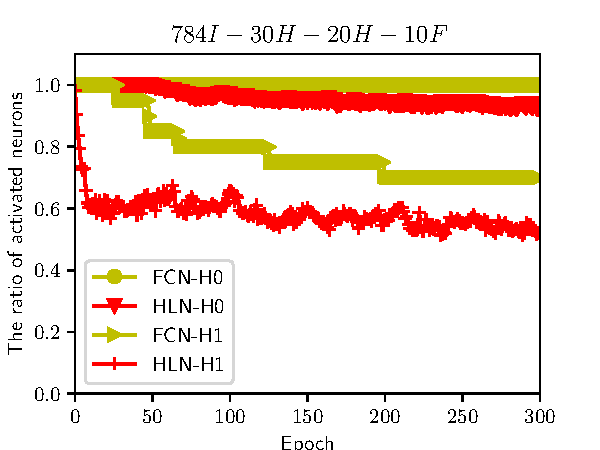
\includegraphics[width=60mm]{mnist_training_sparsity_4}
		\label{fig:6:d}
	}
	\caption{
		Neuron activation sparsity 
		on MNIST with 4 different 
		network models: H0 denotes
		the first hidden layer,
		H1 denotes the second hideen
		layer.
		}
	\label{fig:6}
\end{figure}

Observed from Figure~\ref{fig:4:a}, 
where a single hidden layer 
architecture is used,
the FCN requires about 
150-200 epoches to stablize 
at its best test accuracy of 
93\%, however HLN
only takes 4-5 epoches to achieve 
the same test 
accuracy or even higher. 
Thus it is a $40\times$ speed up 
on the training without a sacrifice 
of the
model capability. 
The HLN additionally provides
much higher stablity at all time 
during the entire
training process. 
The reason behind is that
HLN enables 
the network to unsupervisedly
learn the neuron activation 
clustering map(the SOM) of 
every non-output layer
especially the input layer,
along with
the supervised learning. 
Each sample for the input
is more thoroughly taken in use, 
making HLN learn much faster.

In Figure~\ref{fig:4:b} with 
a deeper architecture,
FCN seems fail to learn at all.
In constrast, HLN keeps a fast 
learning. Though HLN seems 
\emph{slow down} a little bit for
the sake of doubling the hidden layers.
The observation follows: a deeper
architecture brings a tougher 
parameter tuning.

In Figure~\ref{fig:4:c}, 
we use a max-pooling with a kernel 
of $1\times 1$,
which equals to the original input as 
in MNIST.
The input dimension of the network
is therefore 4 
times larger than that in 
Figure~(\ref{fig:4:a}).
However,
HLN learns as fast as the one 
with small input
dimension with equal stablity.
Again FCN fails to learn.

In Figure~\ref{fig:4:d}, 
HLN takes about 120
epoches to stalize at its 
best performance but
FCN seems never start to learn.
Compared to Figure~\ref{fig:4:c}, 
the networks have a
deeper architecture, 
making the model more difficult
to learn as expected.  
Compared to Figure~\ref{fig:4:b},
it has a larger input dimension, 
which leads to a
tougher learning too. 
Putting two factors together
turns out more harmful to
the training as we may expect 
in a linear manner.

Figure~\ref{fig:5} further confirms 
the facts
observed from Figure~\ref{fig:4}.
The test accuracy is not improved at all
with deeper architectures,
whereas the training loss is dropping, 
though, at a very slow pace. 
Figure~\ref{fig:6} shows the neuron 
activation sparsity for every hidden 
layer in networks.
Notice that a SOM-embedding output 
in HLNs is used as a sparsity mask 
to control, or more
precisely, to increase the sparsity 
of every hidden layer. 
It's obvious that networks with 
HLN architecture tend to have a higher 
sparsity than the ones without.

\section{Conclusions}
We proposed HLN, a hybrid learning 
architecture for ANNs.
HLN enables ANNs to learn from
labeled and unlabeled data 
simultaneously and separatedly.
We examined experiments on our
synthetic dataset and the MNIST 
benchmark dataset.
As the experiments showed,
ANNs of HLN architecture 
proved better performance in
training eciency and stablity.
In the future, we will investigate
other capabilities of HLN on more
pulic datasets such as CIFAR-10 and
CIFAR-100.

\section*{Acknowledgements}
This project was partially supported 
by Grants from Natural Science 
Foundation of China
\#71671178/ \#91546201/ \#61202321, 
and the open project of the Key Lab 
of Big Data Mining and
Knowledge Management. 
It was also supported by Hainan 
Provincial Department of Science 
and Technology under Grant 
No. ZDKJ2016021, and by 
Guangdong Provincial Science and
Technology Project 
20162016B010127004.

%% References
%%
%% Following citation commands can be used in the body text:
%% Usage of \cite is as follows:
%%   \cite{key}         ==>>  [#]
%%   \cite[chap. 2]{key} ==>> [#, chap. 2]
%%


%% References with BibTeX database:

\bibliographystyle{elsarticle-num}
\bibliography{ref}

\end{document}

%%
%% End of file `procs-template.tex'.
